 \documentclass[12pt, titlepage]{article}
 \usepackage{amsmath, empheq}
 \usepackage{amssymb}
 \usepackage{geometry}
 \geometry{
 	a4paper,
 	total={170mm,257mm},
 	left=20mm,
 	top=20mm,
 }
\usepackage[utf8]{inputenc}
\usepackage{graphicx}
\usepackage[font=small,labelfont=bf]{caption} % Required for specifying captions to tables and figures

\title{Práctica 2\\ 
\large Implementación del algoritmo del Simplex Primal }
\author{Pedro López Sancha, Emilia Vayssier}

\begin{document}
\maketitle

En este trabajo se ha implementado el algoritmo del Simplex Primal en dos lenguajes de programación distintos: C++ y MATLAB. \\
Se programaron dos versiones del algoritmo que difieren en la forma de elegir de la variable no básica de entrada a la base. La primera versión utiliza la Regla de Bland, mientras que la segunda utiliza la Regla del coste reducido más grande. Ambas versiones constan de las Fases I y II. \\
Se resolvieron los problemas planteados utilizando las dos versiones y se presenta una comparación del rendimiento. Los resultados vienen acompañados de la actualización de los valores a cada iteración.
\newpage

\section{Introducción}
\section{Objetivos}
Los objetivos que se plantean para la práctica són:
\begin{enumerate}
\item	Comprender el fundamento teórico del algoritmos del Símplex primal y su aplicación a la resolución de problemas de programación lineal.
\item	Implementar el algoritmo del Símplex primal.
\end{enumerate}
\section{Metologia}
Los objetivos anteriormente propuestos se alcanzarán con la siguiente metodología:
\begin{enumerate}
\item	Se realizará un estudio exhaustivo de los fundamentos de la programación lineal y del algoritmo del Símplex. En su mayor parte, este objetivo se realizará durante la época de estudio de exámenes parciales.
\item	Se implementará el algoritmo del Símplex primal en dos lenguajes de programación, C++ y MATLAB, y se compararán las implementaciones.
\end{enumerate}



\section{Implementación en C++}
A pesar de que se recomendó emplear MATLAB como lenguaje de programación, hemos decidido implementar el algoritmo en C++ como divertimento, y también como práctica para otras asignaturas como Algoritmia.\\
Para ello, primeramente ha sido necesario crear una clase Matriz que permita implementar el algoritmo del Símplex de manera cómoda.\\
Tras depurar el código de la clase Matriz y comprobar su correcto funcionamiento, se ha implementado el Símplex en C++. Esta implementación funciona tan solo con algunos de los problemas propuestos. Más adelantes, damos las razones de por qué creemos que esto sucede.
\subsection{Clase Matriz}
La clase Matriz se ha implementado siguiendo el paradigma de la programación orientada a objetos. En esta sección se discutirá brevemente la estructuración y funcionalidades de la clase Matriz que se emplean en el algoritmo del Símplex.
\begin{itemize}
\item	La matriz internamente se guarda como un vector de vectores. Es por este motivo por el que se emplea el contenedor \textit{vector} de la librería estándar de C++. 
\item	Así mismo, se guardan las dimensiones de la matriz. En cualquier llamada a una función de la clase, si se accede a una posición que no pertenece a la matriz, se devuelve valor nulo.
\item	Las funciones para las operaciones básicas de matrices son:
\begin{itemize}
\item	Producto de una matriz por un escalar: \textit{scalarProduct}.
\item	Suma de matrices: \textit{matrixSum}.
\item	Producto de matrices: \textit{matrixProduct}.
\item	Matriz transpuesta: \textit{transpose}.
\item	Determinante: \textit{determinant}. El determinante se calcula usando menores. Cabe decir que es una manera ineficiente de calcularlo, por ello el tiempo de ejecución para matrices $10\times10$ como las proporcionadas en datos es del orden de 15 segundos. Por lo tanto, las funciones adjunta y inversa no se ejecutan para matrices grandes.
\item	Matriz adjunta:	\textit{adjoint}.
\item	Matriz inversa:	\textit{inverse}. La inversa se calcula como el producto del inverso del determinante por la matriz adjunta transpuesta.
\item	Matriz identidad: \textit{identity}. Devuelve una matriz identidad de la dimensión especificada.
\end{itemize}
\item	Las funciones para la modificación de matrices son:
\begin{itemize}
\item	Inserción de fila y columna: \textit{insertRow} y \textit{insertCol}.
\item	Inserción de matriz en fila y columna: \textit{insertMatrixInRow} y \textit{insertMatrixInCol}, que permiten insertar una matriz de dimensiones adecuadas en una fila o columna especificada.
\item	Reemplazo de fila y columna: \textit{replaceRow} y \textit{replaceCol}.
\item	Redondeo de matriz: \textit{roundMatrix}. Redondea los valores reales al entero más cercano si están a una distancia inferior o igual a la suministrada como parámetro. Esta función es útil ya que en operaciones entre matrices grandes, el cálculo de números reales pierde precisión.
\end{itemize}
\end{itemize}
\subsection{Implementación del Simplex Primal}

El algoritmo del símplex se ha implementado mediante dos archivos, el archivo de cabecera \textit{Simplex.h} que contiene las declaraciones de las funciones, y el archivo de implementación \textit{Simplex.cc}, que contiene las definiciones de dichas funciones. Se ha eligido esta metodología ya que es la recomendad por la comunidad de programación.

\subsubsection{Funciones en la implementación}
Cada paso del algoritmo tiene su propia función. De este modo, el código es más escalable, estructurado, legible y facilita la comprensión. Las funciones declaradas en el archivo de implementación són:
\begin{itemize}
\item	Cálculo de costes reducidos: \textit{computeReducedCosts}, que calcula el vector de costes reducidos y determina si la solución actual es óptima. En caso de que no sea óptima, devuelve el índice $q$ de la variable no básica que debe entrar en la base y su posición en el vector de variables no básicas, según el criterio de selección escogido, que se especifica en los argumentos.
\item	Cálculo de la dirección básica factible: \textit{computeBasicFeasibleDirection}, que calcula la dirección básica factible. También determina si nos encontramos ante un problema ilimitado, buscando una componente negativa del vector.
\item	Cálculo de la longitud de paso: \textit{computeTheta}, que calcula la longitud de paso a lo largo de la dirección básica factible.
\item	Actualización de matrices:	\textit{updateMatrices}, que actualiza los vectores de coeficientes de variables básicas $c_b$ y no básicas $c_n$, la matriz $A_n$ de coeficientes de variables no básicas, y la inversa de la base $B^{-1}$. Esta última se calcula mediante la actualización de la inversa.
\item	Actualización de variables:	\textit{updateVariables}, que actualiza la función objetivo, las componentes de la solución básica factible actual, y el vector de variables básicas y no básicas.
\item	Degeneración de la base: \textit{isDegenerate}, que busca alguna variable nula en el vector de la solución actual.
\item	Información: \textit{printIteration}, que imprime la información relevante sobre la iteración.
\item	Iteración del simplex: \textit{simplexIteration}, que incorpora todas las funciones anteriores y ejecuta una iteración completa. Cada paso de la iteración se ejecuta únicamente si es posible. Por ejemplo, la dirección básica factible tan solo se calcula si la solución actual no es óptima. Tras cada iteración, devuelve un código, denominado \textit{out}, que puede representar uno de los siguientes casos: problema de fase 1 infactible $(-1)$, algoritmo itera con normalidad $(0)$, óptimo del problema $(1)$, problema ilimitado $(2)$, detección de degeneración $(3)$.
\item	Fase 1 y 2: \textit{phase1} y \textit{phase2}. Se explican más detalladamente en el siguiente apartado.
\end{itemize}


\subsubsection{Funcionamiento de la implementación}
Se han implementado las dos fases del Símplex, de modo que el programa resuelve de manera autónoma la fase 1 y, en caso de ser un problema factible, continúa con la fase 2. El funcionamiento general de la implementación es el siguiente:
\begin{itemize}
\item	Dentro de la función \textit{main} se declaran las matrices que representan el problema y se leen desde un archivo de entrada de extensión \textit{txt}. Así mismo, también se declaran las variables que representan la iteración y el código de salida.
\item	Fase 1: a partir de la matriz de coeficientes $A$, genera la matriz del problema de fase 1 insertando la identidad. También crea los vectores de coeficientes de la función objetivo de fase 1, así como el vector de variables básicas y no básicas. Por último, iguala la solución básica factible inicial $X_b$ al vector de términos independientes $b$ y calcula el valor de la función objetivo. A continuación, comienza a iterar el algoritmo. Este itera mientras el código \textit{out} sea $0$. Una vez acaba, si el óptimo de la función objetivo es $z = 0$, o un valor cercano por tolerancia, determina que el problema es factible. En tal caso, retorna la base óptima primal y su inversa.
\item	De nuevo en el \textit{main}, revisa el vector la base en busca de alguna variable artificial. En caso de encontrarla, para la ejecución del algoritmo. En caso de que no, revisa el vector de variables no básicas y elimina las artificiales. 
\item	Fase 2: a partir del vector de variables básicas y no básicas, crea la matriz no básica $A_n$, los vectores de coeficientes de la función objetivo, y calcula el valor de la función objetivo. En lugar de calcular la inversa de la base, recibe la de fase 1. Seguidamente itera el Símplex mientras que el código \textit{out} sea $0$.
\end{itemize}


\subsection{Errores de la implementación}
Como ya se ha mencionado anteriormente, en cálculos entre matrices de dimensiones del orden de $10 \times 10$, la pérdida de precisión en operaciones entre números reales es significativa, y existe una tolerancia a tener en cuenta. Por este motivo, a medida que el algoritmo itera, las matrices con las que opera se alejan más de las que deberían realmente ser. A continuación se muestra un ejemplo de esto:\\

\begin{center}
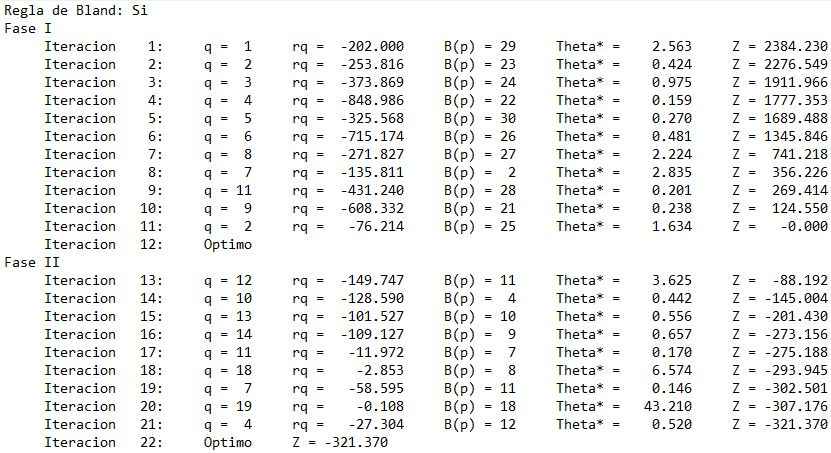
\includegraphics[scale=0.45]{imagenes/p1_bland.JPG}
\captionof{figure}{problema 1, datos 45, con regla de Bland}
\end{center}

\begin{center}
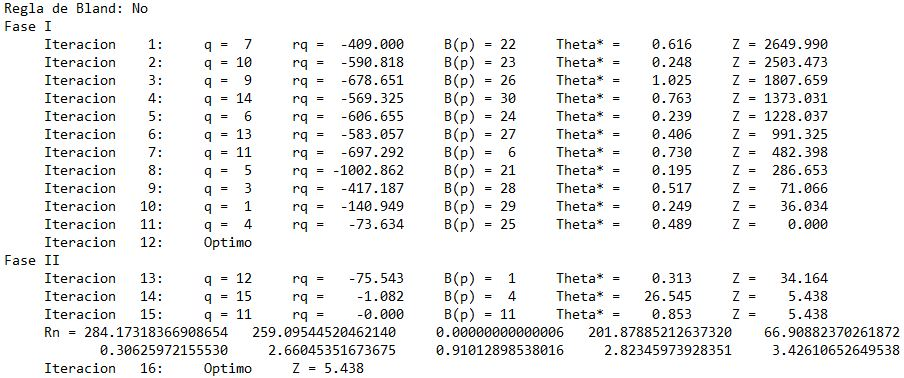
\includegraphics[scale=0.5]{imagenes/p1_no_bland_problema.JPG}
\captionof{figure}{problema 1, datos 45, con coste reducido más negativo}
\end{center}

Aplicando regla de Bland el algoritmo da el mismo óptimo que la solución proporcionada en el conjunto de datos. Sin embargo, aplicando la regla del coste reducido más negativo, llega un momento en el que el vector de costes es no negativo y el algoritmo concluye que es óptimo. Como se puede ver, hay un valor muy cercano a cero, que podría ser negativo por tolerancias. En tal caso, el algoritmo habría seguido iterando.

\begin{center}
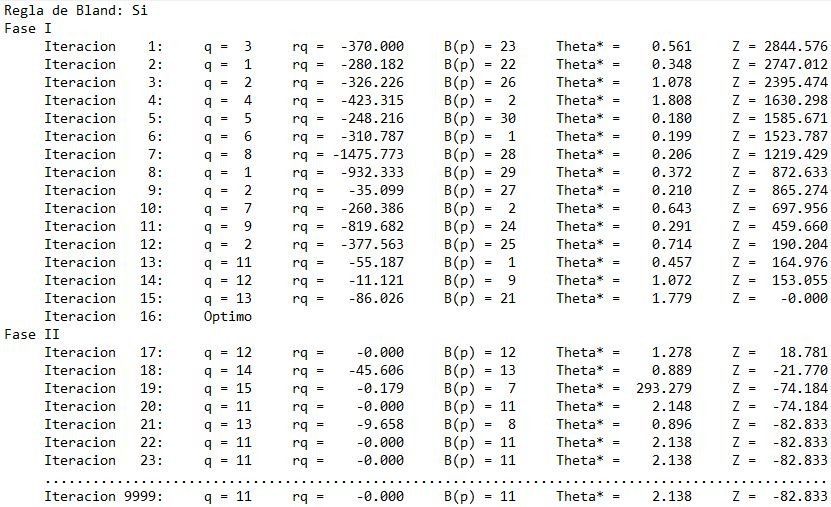
\includegraphics[scale=0.45]{imagenes/p2_bland.JPG}
\captionof{figure}{problema 2, datos 45, con regla de Bland}
\end{center}

\begin{center}
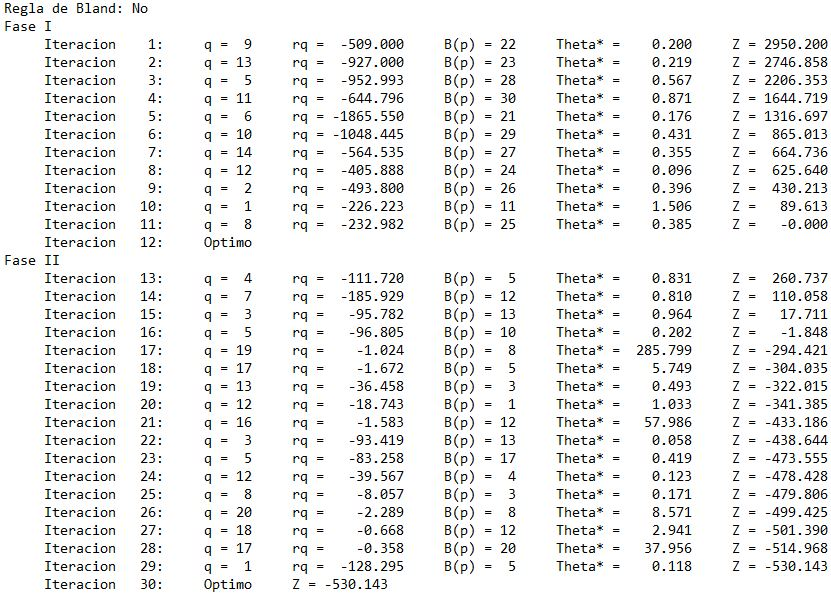
\includegraphics[scale=0.45]{imagenes/p2_no_bland.JPG}
\captionof{figure}{problema 2, datos 45, con coste reducido más negativo}
\end{center}

En este último caso, aplicando regla de Bland, el algoritmo itera indefinidamente, siempre con los mismos datos de iteración. Podemos ver que siempre encuentra un coste reducido negativo pero muy cercano a $0$ que, nuevamente, podría ser positivo por tolerancia. Por el contrario, con coste reducido más negativo, encuentra el óptimo.\\
En cada iteración se ha revisado el funcionamiento del algoritmo, mostrando por pantalla las matrices, y repitiendo los cálculos, sin embargo no se ha encontrado error. El hecho de que la implementación funcione correctamente en determinados casos y en otros falle, sugiere que no es problema de la propia implementación sino, como ya se ha mencionado, de tolerancia.\\
Puesto que la implementación funciona de una manera que no podemos predecir, creemos que no merece la pena probar el algoritmo sobre otros conjuntos de datos, puesto que producirá resultados similares. Por este motivo, no se mostrarán más resultados obtenidos del algoritmo en C++.

\subsection{Posibles mejoras}
La solución al problema de las tolerancias está fuera de nuestros alcance. No obstante, en caso de encontrar o implementar una librería que capaz de resolver este incoveniente, podríamos acabar de desarrollar el código y hacer un programa completamente funcional. Creemos además, que la implementación en C++ sería más eficiente que en MATLAB, por cuestiones relacionadas con las optimizaciones realizadas por el compilador así como por la diferencia en el cálculo de la inversa entre ambos programas.\\
Otra mejora significativa sería en el apartado de la degeneración. En caso de que detectar degeneración y de estar usando la regla del coste reducido más negativo, que no asegura la convergencia del algoritmo, no parar la ejecución del algoritmo. La propuesta es crear una lista con todas las bases por las que el algoritmo ha iterado tras la detección de degeneración. Tras cada iteración, se comprobaría si la base actual ya ha sido visitada. En caso afirmativo, probablemente indicaría que el Símplex está ciclando, y por tanto la ejecución debería acabar o bien cambiar el criterio por la regla de Bland.




\section{Implementación en MATLAB}

\section{Conclusiones}
Las conclusiones que hemos podido extraer tras la realización de la práctica son:
\begin{enumerate}
\item	Hemos aprendido los fundamentos teóricos del Símplex primal y sabemos aplicarlo para resolver un problema de programación lineal. Así mismo, hemos visto que la manera en que se nos ha enseñado y hemos estudiado el algoritmo es más sencilla y bella que el método del tablón del Símplex, 
\item	Hemos conseguido desarrollar el Símplex en MATLAB y en C++, y hemos observado diferencias significativas entre ambas implementaciones. En la primera, el algoritmo funciona de manera correcta. El código resultante tiene un sintaxis semejante al lenguaje matemático, por tanto es fácilmente comprensible y la extensión del programa es reducida. Por el contrario, la implementación en C++ ha sido más costosa y únicamente funciona en determinados problemas. Concluimos, por lo tanto, que es recomendable implementarlo en un lenguaje pensado específicamente para el trabajo de objetos matemáticos, como puede ser MATLAB u Octave.
\end{enumerate}

\end{document}